\section{Einleitung}

In diesem Versuch soll das Verhalten und die Struktur eines Silizium-Streifensensors untersucht werden. Streifensensoren werden in der Teilchenphysik eingesetzt um mit schnellem Antwortverhalten die Spuren von Teilchen in Teilchenbeschleunigerexperimenten zu vermessen. Ein Beispiel für ein solches Experiment ist ATLAS am Large Hadron Collider in der Schweiz, dass in der zweiten Lage des Spurfindungssystems Streifensensoren nutzt, die den hier benutzen sehr ähnlich sind.


\section{Theorie}
\label{sec:Theorie}

Folgendes orientiert sich an \cite{anleitung} und \cite{goessling}.

\subsection{Halbleiter}

Der genutzte Silizium-Streifensensor ist ein Halbleiterdetektor. Halbleiter sind Elemente oder Verbindungen, die bei $T = \SI{0}{\kelvin}$ keinen Strom leiten. Ihre Leitfähigkeit lässt sich aber leicht manipulieren durch Anregung oder Einbringen von Fremdatomen. Diese Steuerung macht sie interessant für viele Einsatzgebiete.
Sie unterscheiden sich von Leitern und Isolatoren durch die Größe der Bandlücke zwischen Valenzband und Leitungsband. Während die Bänder sich bei Leitern überschneiden, beträgt die Größe der Bandlücke bei Isolatoren je nach Definition circa $\SI{10}{\electronvolt}$ und liegt bei Halbleitern bei wenigen $\si{\electronvolt}$. Die Bandlücke bei reinem Silizium beträgt beispielsweise $\SI{1.1}{\electronvolt}$. Das Bandschema im nicht angeregten Zustand eines Halbleiters ist in Abbildung \ref{fig:bandmodell} zu sehen.

\begin{figure}
  \centering
  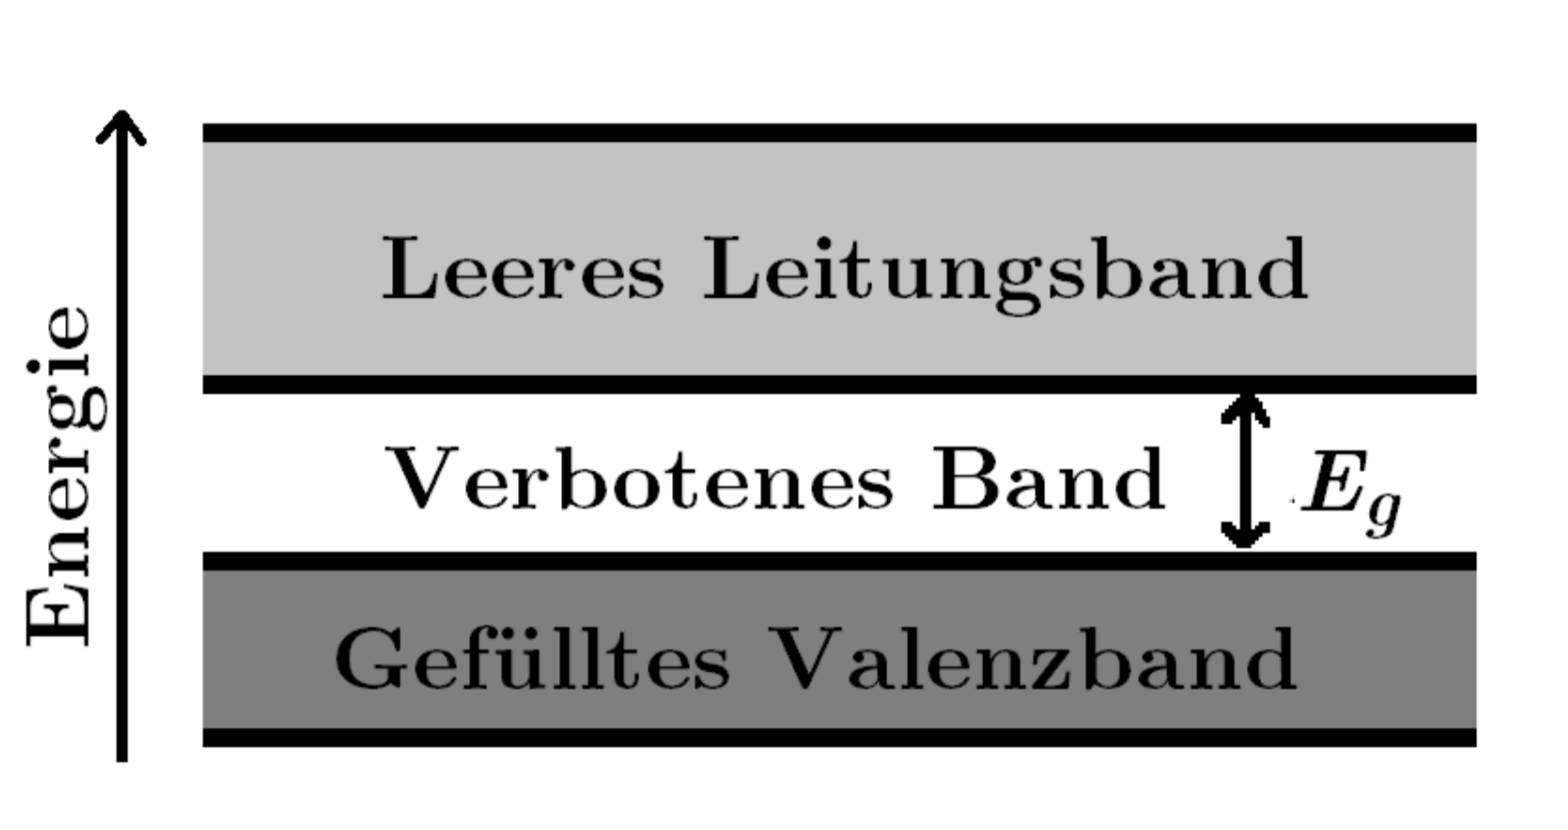
\includegraphics[height=6cm]{TimosAufrisse/bandmodell.png}
  \caption{Bandschema eines Halbleiters\cite{anleitung}.}
  \label{fig:bandmodell}
\end{figure}

Um die Leitfähigkeit von Halbleitern gezielt zu steigern werden sie mit Fremdatomen dotiert. Das hier verwendete Silizium besitzt vier Valenzelektronen. Nun wird hier Arsen als Donator mit fünf Valenzelektronen eingeführt. Dadurch ist ein Elektron nicht an der Bindung beteiligt und kann als Ladungsträger dienen. Außerdem kann noch Bor als Akzeptor mit drei Valenzelektronen eingeführt werden. So existiert eine elektronfreie Stelle ein Loch als Ladungsträger. Dargestellt ist dies in Abbildung \ref{fig:dotierung}.

\begin{figure}
  \centering
  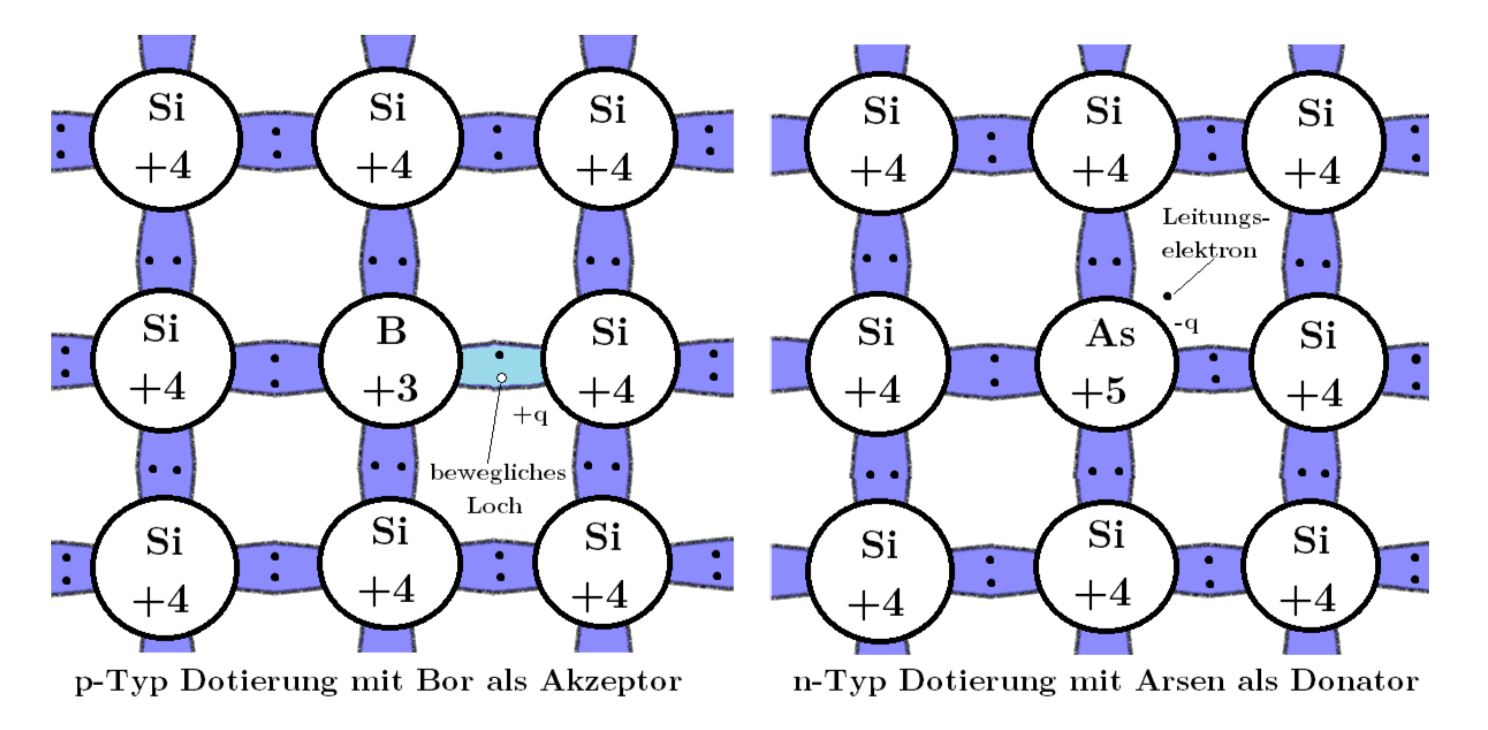
\includegraphics[height=6cm]{TimosAufrisse/dotierung.png}
  \caption{Skizze der zwei hier verwendeten Dotierungsarten \cite{anleitung}.}
  \label{fig:dotierung}
\end{figure}

Wenn ein mit Donatoren n-dotierter Halbleiter verbunden wird mit einem mit Akzeptoren p-dotierten bildet sich eine Depletionszone aus, da die freien Elektronen mit den Löchern kombinieren und so geladene Atomrümpfe hinterlassen. Dies ist in Abbildung \ref{fig:pnuebergang} zu sehen.

\begin{figure}
  \centering
  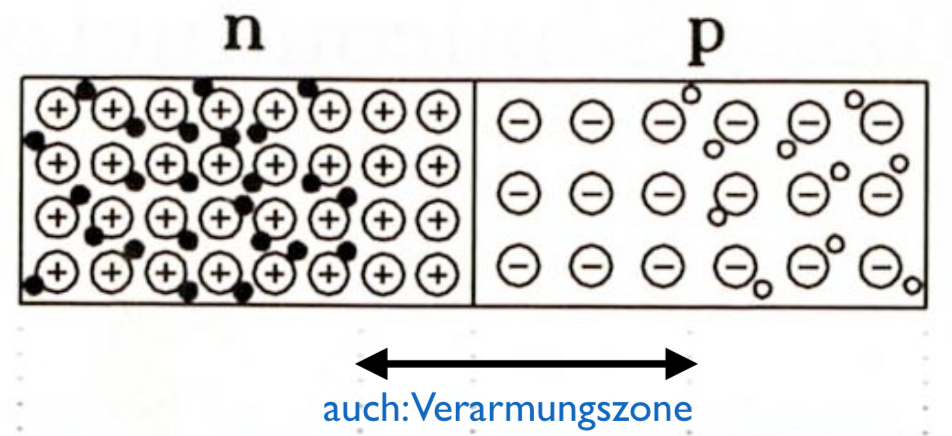
\includegraphics[height=4cm]{TimosAufrisse/pnuebergang.png}
  \caption{Darstellung der Verarmungszone bei einer Diode \cite{goessling}.}
  \label{fig:pnuebergang}
\end{figure}

Um hier als Detektor zu dienen, wird an den pn-Halbleiter noch eine Spannung so angelegt, dass sie die Depletionszone noch vergrößert.
Wenn die Depletionszone den gesamten Halbleiter ausmacht, sollte theoretisch kein Strom mehr fließen, da keine freien Ladungsträger vorhanden sind. Ein einfallendes ionisierendes Teilchen erzeugt Elektronen-Loch-Paare in dieser Zone, die als Ladungsfluss detektiert werden können.

\subsection{Einfallende Strahlung}

Die hier zu detektierende Strahlung stammt aus dem Zerfall:
\begin{align}
  \ce{Sr^{90} ->[$\beta^-$] Y^{90} ->[$\beta^-$] Zr^{90}}. \label{eqn:zerfall}
\end{align}
Die detektierten Teilchen in diesem Versuch sind die Elektronen aus der Umwandlung eines Neutrons in ein Proton unter Aussendung eines Elektrons und eines Antineutrinos:
\begin{align*}
  n \to p + e^- + \bar \nu.
\end{align*}
Dabei ist die Energieverteilung des Elektrons kontinuierlich, da die freiwerdende Energie beim Neutronzerfall zufällig auf Elektron und Neutrino aufgeteilt wird. Die Energieverteilung hat dann die Form aus Abbildung \ref{fig:elektronenergie}.
\begin{figure}
  \centering
  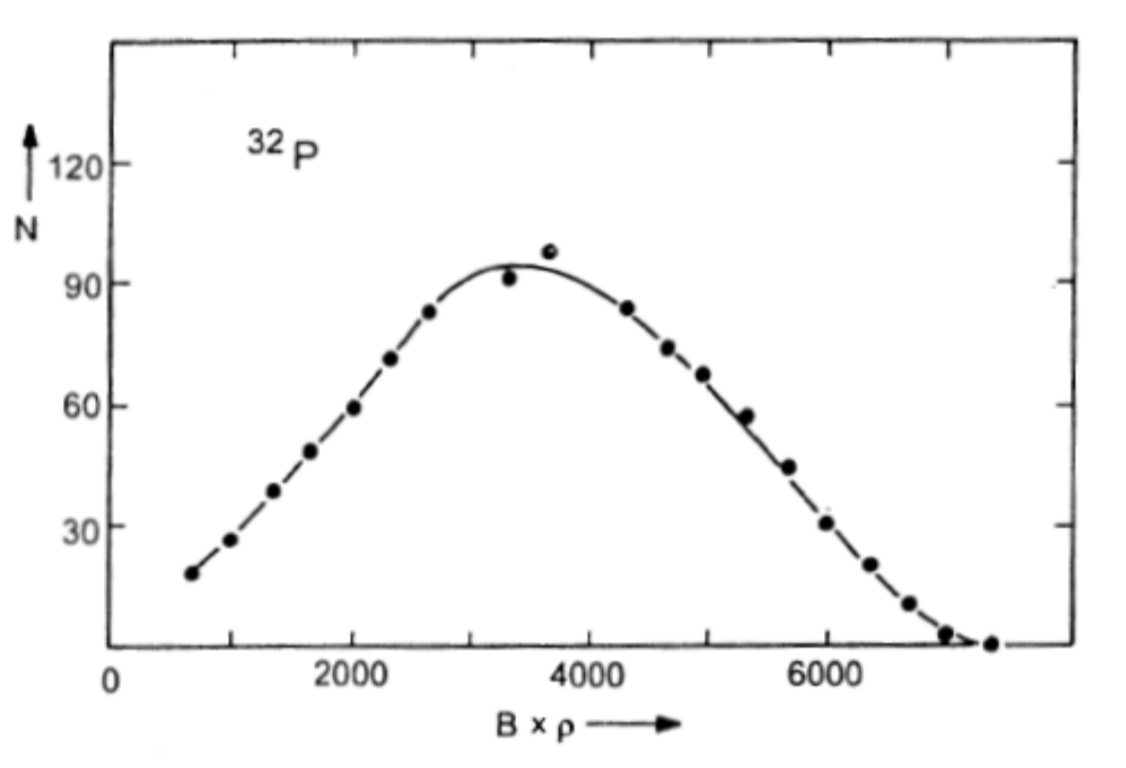
\includegraphics[height=4cm]{TimosAufrisse/elektronenenergie.png}
  \caption{Energieverteilung des Elektrons \cite{anleitung}.}
  \label{fig:elektronenergie}
\end{figure}
Von Interesse sind in diesem Versuch nur die Elektronen aus dem ersten Teil des Zerfalls aus \eqref{eqn:zerfall}. Da aber der zweite
Teil bei einer wesentlich höheren maximalen Emissionsenergie abläuft ($E = \SI{2.28}{\mega\electronvolt}$ im Vergleich zu $E = \SI{0.546}{\mega\electronvolt}$ bei
$\ce{Sr^{90} ->[$\beta^-$] Y^{90}}$), kann durch Schneiden auf der Energie, der Einfluss auf die Messung reduziert werden.

Die ausgesandten Elektronen wechselwirken beim durchdringen des Detektors mit der Materie und verlieren so einen Teil ihrer Energie.
Sie stoßen entweder elastisch und werden gestreut oder inelastisch und lösen Hüllenelektronen aus, dessen Ladungsfluss dann detektiert wird.
Die Energiedeposition im Streifendetektor ist nicht wie bei dickeren Materialien gaußverteilt, sondern folgt der Landauverteilung; schematisch gezeigt in Abbildung \ref{fig:energiedepositionElektron}. Ein Grund dafür ist, dass die Elektronen nicht ihre geamte Energie deponieren.
\begin{figure}
  \centering
  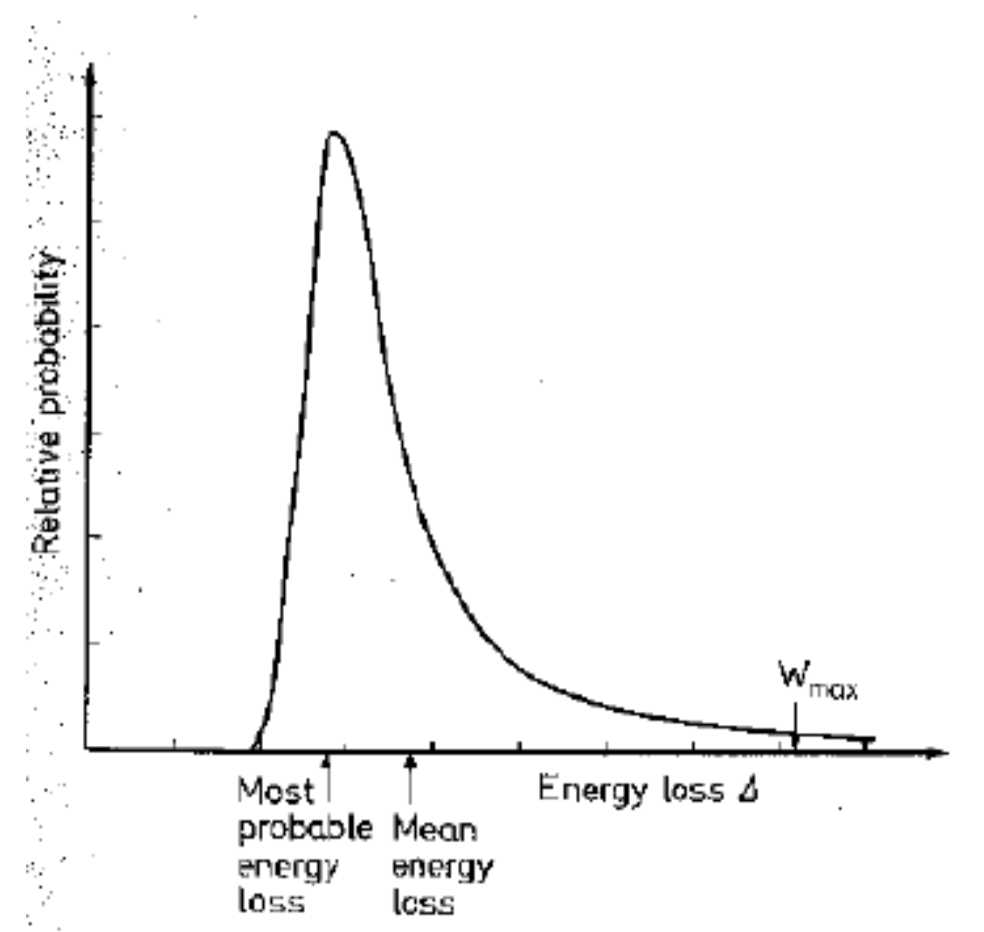
\includegraphics[height=4cm]{TimosAufrisse/energiedepositionElektron.png}
  \caption{Energiedeposition des Elektrons in einem dünnen Sensor \cite{anleitung}.}
  \label{fig:energiedepositionElektron}
\end{figure}

\subsection{Antwortverhalten des Detektors}

Der Detektor gibt die deponierte Energie des einfallenden Elektrons in ADC-Charges an. Die Umrechnung in Elektronenvolt erfolgt über eine polynomielle Annäherung, die aus einer Kalibrationsrechnung folgt. Außerdem fließt in die Rechnung das Wissen ein, dass zur Erzeugung eines Elektronen-Loch-Paares eine Energie von $\SI{3.6}{\electronvolt}$ von Nöten sind.

Der ADC-Count für ein Signal $k$ und den Streifen $i$ setzt sich wie folgt zusammen:
\begin{align}
  \text{ADC}(i, k) = \symup{P}(i) + \symup{D}(k) + \text{Signal}{i, k}.
\end{align}
Dabei sind die Pedestals der durchschnittliche Offset der Streifen ohne Signal:
\begin{align}
  \symup{P}(i) = \frac{1}{N} \sum_{k=1}^N \text{ADC}(i, k).
\end{align}
Die Streifen sind so eingestellt, dass ihr Offset bei \num{500} ADC-Counts liegt.
Der Common Mode Shift auch Common Noise D$(k)$ ist ein globales Rauschen, das im allgemeinen gaußverteilt ist mit dem Mittelwert Null. Es berechnet sich wie folgt:
\begin{align}
  \symup{D}(k) = \frac{1}{128} \sum_{i=1}^{128} (\text{ADC}(i, k) - \symup{P}(i)).
\end{align}
Zuletzt lässt sich noch das Rauschen jedes einzelnen Streifens nach
\begin{align}
  \text{Noise}(i) = \sqrt{\frac{1}{N-1} \sum_{k=1}^N(\text{ADC}(i, k) - \symup{P}(i) - \symup{D}(k))^2}
\end{align}
berechnen.

% \subsection{Fehlerrechnung}
%
% Für die Fehlerfortpflanzung bei Gleichungen mit $N$ fehlerbehafteten Größen
% wird jeweils die Formel zur Gaußschen Fehlerfortpflanzung
%
% \begin{equation*}
%   \sigma = \sqrt{\sum_{i=1}^{N}\biggl(\frac{\partial f(x_{\g{i}})}{\partial x_{\g{i}}}
%   \sigma_{\g{i}}\biggr)^2}
% \end{equation*}
% mit der jeweiligen Funktion $f(x_{\g{i}})$, den Messgrößen $x_{\g{i}}$ und den
% zugehörigen Fehlern $\sigma_i$ verwendet.
% Zur Berechnung des arithmetischen Mittels von $N$ Messwerten wird jeweils die
% Formel
%
% \begin{equation*}
%   \bar{x} = \frac{1}{N}\sum_{i=1}^{N}x_{\g{i}}
% \end{equation*}
% mit den Messwerten $x_i$ benutzt.
% Die Standardabweichung des Mittelwerts wird jeweils mit der Gleichung
%
% \begin{equation*}
%   \bar{\sigma} = \sqrt{\frac{1}{N-1}\sum_{i=1}^{N}(x_{\g{i}} - \bar{x})^2}
% \end{equation*}
% mit den $N$ Messwerten $x_i$ berechnet.




\cite{anleitung}
